\chapter{Renormalization: Putting It All Together}
\section{Renormalization Example: Compton Scattering}
The additional 2nd order in $\alpha_0$(4th order in $e_0$) amplitude contributions we need to include. The Feynman diagrams for all of these are shown in Fig. (\ref{fig:compton-tree-2nd})
\begin{figure}[H]
    \centering
\tikzset{every picture/.style={line width=0.75pt}} %set default line width to 0.75pt        
%x=0.75pt,y=0.75pt,yscale=-1,xscale=1
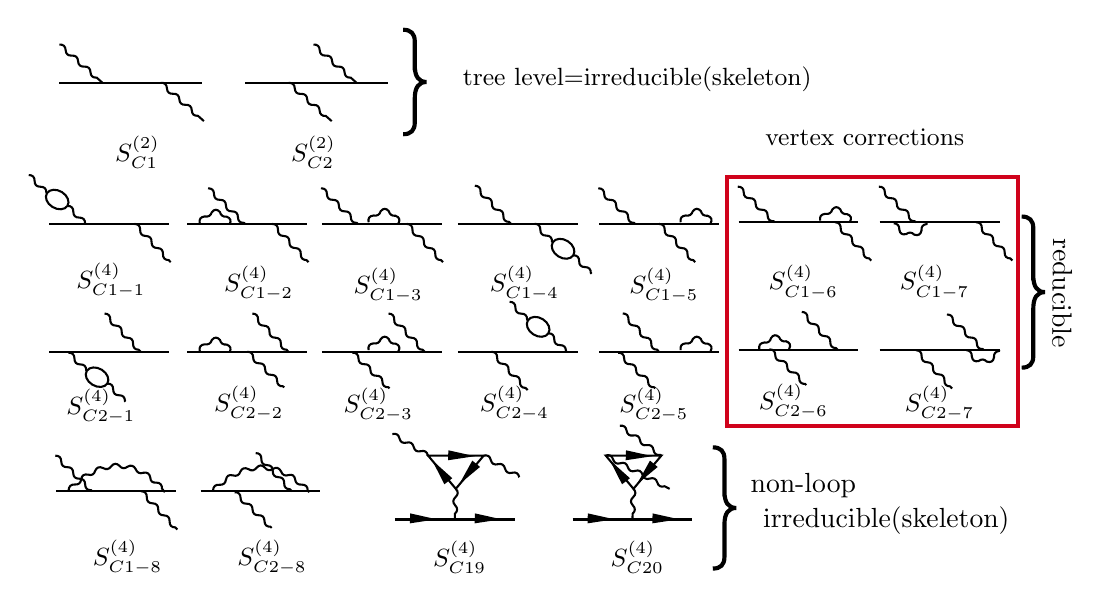
\begin{tikzpicture}[x=0.75pt,y=0.75pt,yscale=-0.8,xscale=0.8]
%uncomment if require: \path (0,367); %set diagram left start at 0, and has height of 367

%Straight Lines [id:da9913352016626935] 
\draw    (32,49) -- (118,49) ;
%Straight Lines [id:da7191403312933694] 
\draw    (93,49) .. controls (95.35,48.86) and (96.6,49.97) .. (96.74,52.32) .. controls (96.88,54.67) and (98.13,55.78) .. (100.48,55.64) .. controls (102.83,55.49) and (104.08,56.6) .. (104.22,58.95) .. controls (104.36,61.3) and (105.61,62.41) .. (107.96,62.27) .. controls (110.31,62.13) and (111.56,63.24) .. (111.7,65.59) .. controls (111.84,67.94) and (113.09,69.05) .. (115.44,68.91) -- (119,72.07) -- (119,72.07) ;
%Straight Lines [id:da08993792222767738] 
\draw    (32,26) .. controls (34.35,25.86) and (35.6,26.97) .. (35.74,29.32) .. controls (35.88,31.67) and (37.13,32.78) .. (39.48,32.64) .. controls (41.83,32.49) and (43.08,33.6) .. (43.22,35.95) .. controls (43.36,38.3) and (44.61,39.41) .. (46.96,39.27) .. controls (49.31,39.13) and (50.56,40.24) .. (50.7,42.59) .. controls (50.84,44.94) and (52.09,46.05) .. (54.44,45.91) -- (58,49.07) -- (58,49.07) ;
%Straight Lines [id:da02774886494727591] 
\draw    (144,49) -- (230,49) ;
%Straight Lines [id:da2592044129053318] 
\draw    (170,49.07) .. controls (172.35,48.92) and (173.6,50.03) .. (173.74,52.38) .. controls (173.88,54.73) and (175.13,55.84) .. (177.48,55.7) .. controls (179.83,55.56) and (181.08,56.67) .. (181.22,59.02) .. controls (181.36,61.37) and (182.61,62.48) .. (184.96,62.34) .. controls (187.31,62.2) and (188.56,63.31) .. (188.7,65.66) .. controls (188.84,68.01) and (190.09,69.12) .. (192.44,68.98) -- (196,72.13) -- (196,72.13) ;
%Straight Lines [id:da8766317872451554] 
\draw    (185,26) .. controls (187.35,25.86) and (188.6,26.97) .. (188.74,29.32) .. controls (188.88,31.67) and (190.13,32.78) .. (192.48,32.64) .. controls (194.83,32.49) and (196.08,33.6) .. (196.22,35.95) .. controls (196.36,38.3) and (197.61,39.41) .. (199.96,39.27) .. controls (202.31,39.13) and (203.56,40.24) .. (203.7,42.59) .. controls (203.84,44.94) and (205.09,46.05) .. (207.44,45.91) -- (211,49.07) -- (211,49.07) ;
%Shape: Brace [id:dp44402891522643273] 
\draw  [line width=1.5]  (239,80) .. controls (243.67,80) and (246,77.67) .. (246,73) -- (246,58.53) .. controls (246,51.86) and (248.33,48.53) .. (253,48.53) .. controls (248.33,48.53) and (246,45.2) .. (246,38.53)(246,41.53) -- (246,24.07) .. controls (246,19.4) and (243.67,17.07) .. (239,17.07) ;
%Straight Lines [id:da11968005974247198] 
\draw    (26,134) -- (98.16,134) ;
%Straight Lines [id:da5501206344201499] 
\draw    (77.18,134) .. controls (79.54,134.07) and (80.69,135.28) .. (80.62,137.63) .. controls (80.55,139.99) and (81.7,141.2) .. (84.06,141.27) .. controls (86.41,141.34) and (87.56,142.55) .. (87.49,144.9) .. controls (87.43,147.25) and (88.58,148.46) .. (90.93,148.53) .. controls (93.28,148.6) and (94.43,149.81) .. (94.36,152.16) .. controls (94.29,154.52) and (95.44,155.73) .. (97.8,155.8) -- (99,157.07) -- (99,157.07) ;
%Straight Lines [id:da28185276675918847] 
\draw    (36.83,123.14) .. controls (39.18,123.13) and (40.36,124.31) .. (40.37,126.66) .. controls (40.38,129.02) and (41.56,130.2) .. (43.92,130.19) .. controls (46.27,130.18) and (47.45,131.36) .. (47.46,133.71) -- (47.82,134.07) -- (47.82,134.07) ;
%Shape: Ellipse [id:dp8456750677522806] 
\draw   (24.49,115.5) .. controls (26.07,113.03) and (30.12,112.74) .. (33.53,114.85) .. controls (36.93,116.97) and (38.41,120.67) .. (36.83,123.14) .. controls (35.24,125.6) and (31.2,125.89) .. (27.79,123.78) .. controls (24.38,121.67) and (22.91,117.96) .. (24.49,115.5) -- cycle ;
%Straight Lines [id:da4732096651028763] 
\draw    (13.5,104.57) .. controls (15.86,104.56) and (17.04,105.73) .. (17.05,108.09) .. controls (17.05,110.45) and (18.23,111.63) .. (20.59,111.62) .. controls (22.95,111.61) and (24.13,112.78) .. (24.14,115.14) -- (24.49,115.5) -- (24.49,115.5) ;
%Straight Lines [id:da4855480934643672] 
\draw    (109,134) -- (181.16,134) ;
%Straight Lines [id:da6992146282607298] 
\draw    (160.18,134) .. controls (162.54,134.07) and (163.69,135.28) .. (163.62,137.63) .. controls (163.55,139.99) and (164.7,141.2) .. (167.06,141.27) .. controls (169.41,141.34) and (170.56,142.55) .. (170.49,144.9) .. controls (170.43,147.25) and (171.58,148.46) .. (173.93,148.53) .. controls (176.28,148.6) and (177.43,149.81) .. (177.36,152.16) .. controls (177.29,154.52) and (178.44,155.73) .. (180.8,155.8) -- (182,157.07) -- (182,157.07) ;
%Straight Lines [id:da841197605800111] 
\draw    (121.5,112.57) .. controls (123.86,112.52) and (125.06,113.68) .. (125.1,116.04) .. controls (125.15,118.39) and (126.35,119.55) .. (128.7,119.5) .. controls (131.05,119.46) and (132.25,120.62) .. (132.3,122.97) .. controls (132.35,125.32) and (133.55,126.48) .. (135.9,126.44) .. controls (138.25,126.4) and (139.45,127.56) .. (139.5,129.91) .. controls (139.55,132.26) and (140.75,133.42) .. (143.1,133.38) -- (143.82,134.07) -- (143.82,134.07) ;
%Curve Lines [id:da6500732030699601] 
\draw    (116.5,133.57) .. controls (116.03,131.13) and (117.02,129.78) .. (119.47,129.51) .. controls (121.68,129.91) and (123.11,129.06) .. (123.78,126.95) .. controls (125.35,125.02) and (126.98,124.98) .. (128.65,126.85) .. controls (129.22,128.93) and (130.58,129.87) .. (132.72,129.66) .. controls (135.06,130.53) and (135.64,132.07) .. (134.47,134.27) -- (134.5,134.57) ;
%Straight Lines [id:da46437398008753494] 
\draw    (190,134) -- (262.16,134) ;
%Straight Lines [id:da3433701627732737] 
\draw    (241.18,134) .. controls (243.54,134.07) and (244.69,135.28) .. (244.62,137.63) .. controls (244.55,139.99) and (245.7,141.2) .. (248.06,141.27) .. controls (250.41,141.34) and (251.56,142.55) .. (251.49,144.9) .. controls (251.43,147.25) and (252.58,148.46) .. (254.93,148.53) .. controls (257.28,148.6) and (258.43,149.81) .. (258.36,152.16) .. controls (258.29,154.52) and (259.44,155.73) .. (261.8,155.8) -- (263,157.07) -- (263,157.07) ;
%Straight Lines [id:da5247983359996137] 
\draw    (189.5,112.57) .. controls (191.86,112.52) and (193.06,113.68) .. (193.1,116.04) .. controls (193.15,118.39) and (194.35,119.55) .. (196.7,119.5) .. controls (199.05,119.46) and (200.25,120.62) .. (200.3,122.97) .. controls (200.35,125.32) and (201.55,126.48) .. (203.9,126.44) .. controls (206.25,126.4) and (207.45,127.56) .. (207.5,129.91) .. controls (207.55,132.26) and (208.75,133.42) .. (211.1,133.38) -- (211.82,134.07) -- (211.82,134.07) ;
%Curve Lines [id:da8667530509992772] 
\draw    (218.18,133) .. controls (217.72,130.56) and (218.71,129.21) .. (221.15,128.94) .. controls (223.36,129.34) and (224.8,128.49) .. (225.47,126.38) .. controls (227.04,124.45) and (228.66,124.42) .. (230.33,126.28) .. controls (230.9,128.37) and (232.26,129.31) .. (234.41,129.1) .. controls (236.75,129.97) and (237.33,131.51) .. (236.15,133.7) -- (236.18,134) ;
%Straight Lines [id:da12457167082409482] 
\draw    (272,134) -- (344.16,134) ;
%Straight Lines [id:da10716887595236413] 
\draw    (282.18,111) .. controls (284.54,111.07) and (285.69,112.28) .. (285.62,114.63) .. controls (285.55,116.99) and (286.7,118.2) .. (289.06,118.27) .. controls (291.41,118.34) and (292.56,119.55) .. (292.49,121.9) .. controls (292.43,124.25) and (293.58,125.46) .. (295.93,125.53) .. controls (298.28,125.6) and (299.43,126.81) .. (299.36,129.16) .. controls (299.29,131.52) and (300.44,132.73) .. (302.8,132.8) -- (304,134.07) -- (304,134.07) ;
%Straight Lines [id:da32692714545102763] 
\draw    (341.49,152.88) .. controls (343.84,152.89) and (345.01,154.08) .. (345,156.44) .. controls (344.98,158.8) and (346.15,159.99) .. (348.51,160) .. controls (350.87,160.01) and (352.04,161.19) .. (352.03,163.55) -- (352.5,164.03) -- (352.5,164.03) ;
%Shape: Ellipse [id:dp7823172366742522] 
\draw   (329.13,145.08) .. controls (330.71,142.57) and (334.77,142.27) .. (338.18,144.43) .. controls (341.59,146.58) and (343.07,150.37) .. (341.49,152.88) .. controls (339.9,155.4) and (335.85,155.69) .. (332.43,153.53) .. controls (329.02,151.38) and (327.54,147.6) .. (329.13,145.08) -- cycle ;
%Straight Lines [id:da0940779108375066] 
\draw    (318.12,133.93) .. controls (320.47,133.94) and (321.64,135.13) .. (321.63,137.49) .. controls (321.62,139.84) and (322.79,141.03) .. (325.14,141.04) .. controls (327.5,141.05) and (328.67,142.24) .. (328.65,144.6) -- (329.13,145.08) -- (329.13,145.08) ;
%Straight Lines [id:da5916423830815812] 
\draw    (357,134) -- (429.16,134) ;
%Straight Lines [id:da357939765370912] 
\draw    (393.08,134) .. controls (395.43,134.07) and (396.58,135.28) .. (396.52,137.63) .. controls (396.45,139.98) and (397.6,141.2) .. (399.95,141.27) .. controls (402.3,141.34) and (403.45,142.55) .. (403.39,144.9) .. controls (403.32,147.25) and (404.47,148.46) .. (406.82,148.53) .. controls (409.17,148.6) and (410.32,149.81) .. (410.26,152.16) .. controls (410.19,154.51) and (411.34,155.73) .. (413.69,155.8) -- (414.9,157.07) -- (414.9,157.07) ;
%Straight Lines [id:da7835084803189419] 
\draw    (356.5,112.57) .. controls (358.86,112.52) and (360.06,113.68) .. (360.1,116.04) .. controls (360.15,118.39) and (361.35,119.55) .. (363.7,119.5) .. controls (366.05,119.46) and (367.25,120.62) .. (367.3,122.97) .. controls (367.35,125.32) and (368.55,126.48) .. (370.9,126.44) .. controls (373.25,126.4) and (374.45,127.56) .. (374.5,129.91) .. controls (374.55,132.26) and (375.75,133.42) .. (378.1,133.38) -- (378.82,134.07) -- (378.82,134.07) ;
%Curve Lines [id:da5565886989883443] 
\draw    (406.16,133) .. controls (405.69,130.56) and (406.68,129.21) .. (409.13,128.94) .. controls (411.34,129.34) and (412.77,128.49) .. (413.44,126.38) .. controls (415.01,124.45) and (416.64,124.42) .. (418.31,126.28) .. controls (418.88,128.37) and (420.24,129.31) .. (422.38,129.1) .. controls (424.72,129.97) and (425.3,131.51) .. (424.13,133.7) -- (424.16,134) ;
%Straight Lines [id:da36013246610112726] 
\draw    (441,133) -- (513.16,133) ;
%Straight Lines [id:da6975736791102584] 
\draw    (499.08,133) .. controls (501.43,133.07) and (502.58,134.28) .. (502.52,136.63) .. controls (502.45,138.98) and (503.6,140.2) .. (505.95,140.27) .. controls (508.3,140.34) and (509.45,141.55) .. (509.39,143.9) .. controls (509.32,146.25) and (510.47,147.46) .. (512.82,147.53) .. controls (515.17,147.6) and (516.32,148.81) .. (516.26,151.16) .. controls (516.19,153.51) and (517.34,154.73) .. (519.69,154.8) -- (520.9,156.07) -- (520.9,156.07) ;
%Straight Lines [id:da37417266063176546] 
\draw    (440.5,111.57) .. controls (442.86,111.52) and (444.06,112.68) .. (444.1,115.04) .. controls (444.15,117.39) and (445.35,118.55) .. (447.7,118.5) .. controls (450.05,118.46) and (451.25,119.62) .. (451.3,121.97) .. controls (451.35,124.32) and (452.55,125.48) .. (454.9,125.44) .. controls (457.25,125.4) and (458.45,126.56) .. (458.5,128.91) .. controls (458.55,131.26) and (459.75,132.42) .. (462.1,132.38) -- (462.82,133.07) -- (462.82,133.07) ;
%Curve Lines [id:da7812754413847967] 
\draw    (490.16,132) .. controls (489.69,129.56) and (490.68,128.21) .. (493.13,127.94) .. controls (495.34,128.34) and (496.77,127.49) .. (497.44,125.38) .. controls (499.01,123.45) and (500.64,123.42) .. (502.31,125.28) .. controls (502.88,127.37) and (504.24,128.31) .. (506.38,128.1) .. controls (508.72,128.97) and (509.3,130.51) .. (508.13,132.7) -- (508.16,133) ;
%Straight Lines [id:da4362628175300576] 
\draw    (526,133) -- (598.16,133) ;
%Straight Lines [id:da6695958117269168] 
\draw    (584.08,133) .. controls (586.43,133.07) and (587.58,134.28) .. (587.52,136.63) .. controls (587.45,138.98) and (588.6,140.2) .. (590.95,140.27) .. controls (593.3,140.34) and (594.45,141.55) .. (594.39,143.9) .. controls (594.32,146.25) and (595.47,147.46) .. (597.82,147.53) .. controls (600.17,147.6) and (601.32,148.81) .. (601.26,151.16) .. controls (601.19,153.51) and (602.34,154.73) .. (604.69,154.8) -- (605.9,156.07) -- (605.9,156.07) ;
%Straight Lines [id:da9736049581086236] 
\draw    (525.5,111.57) .. controls (527.86,111.52) and (529.06,112.68) .. (529.1,115.04) .. controls (529.15,117.39) and (530.35,118.55) .. (532.7,118.5) .. controls (535.05,118.46) and (536.25,119.62) .. (536.3,121.97) .. controls (536.35,124.32) and (537.55,125.48) .. (539.9,125.44) .. controls (542.25,125.4) and (543.45,126.56) .. (543.5,128.91) .. controls (543.55,131.26) and (544.75,132.42) .. (547.1,132.38) -- (547.82,133.07) -- (547.82,133.07) ;
%Curve Lines [id:da5212602650402646] 
\draw    (534.5,133.57) .. controls (536.83,133.86) and (537.93,135.15) .. (537.81,137.44) .. controls (538.2,139.86) and (539.57,140.75) .. (541.94,140.11) .. controls (543.71,138.82) and (545.33,138.95) .. (546.81,140.48) .. controls (549.26,141.25) and (550.71,140.41) .. (551.17,137.98) .. controls (550.96,135.73) and (551.97,134.44) .. (554.2,134.1) -- (554.5,133.57) ;
%Shape: Brace [id:dp28652232649113674] 
\draw  [line width=1.5]  (611.5,220.57) .. controls (616.17,220.57) and (618.5,218.24) .. (618.5,213.57) -- (618.5,185.07) .. controls (618.5,178.4) and (620.83,175.07) .. (625.5,175.07) .. controls (620.83,175.07) and (618.5,171.74) .. (618.5,165.07)(618.5,168.07) -- (618.5,136.57) .. controls (618.5,131.9) and (616.17,129.57) .. (611.5,129.57) ;
%Straight Lines [id:da19191767304584262] 
\draw    (26,211) -- (98.16,211) ;
%Straight Lines [id:da9965842822992208] 
\draw    (59.18,188) .. controls (61.54,188.07) and (62.69,189.28) .. (62.62,191.63) .. controls (62.55,193.99) and (63.7,195.2) .. (66.06,195.27) .. controls (68.41,195.34) and (69.56,196.55) .. (69.49,198.9) .. controls (69.43,201.25) and (70.58,202.46) .. (72.93,202.53) .. controls (75.28,202.6) and (76.43,203.81) .. (76.36,206.16) .. controls (76.29,208.52) and (77.44,209.73) .. (79.8,209.8) -- (81,211.07) -- (81,211.07) ;
%Straight Lines [id:da6806195731688666] 
\draw    (60.83,230.14) .. controls (63.18,230.13) and (64.36,231.31) .. (64.37,233.66) .. controls (64.38,236.02) and (65.56,237.2) .. (67.92,237.19) .. controls (70.27,237.18) and (71.45,238.36) .. (71.46,240.71) -- (71.82,241.07) -- (71.82,241.07) ;
%Shape: Ellipse [id:dp8162588386395363] 
\draw   (48.49,222.5) .. controls (50.07,220.03) and (54.12,219.74) .. (57.53,221.85) .. controls (60.93,223.97) and (62.41,227.67) .. (60.83,230.14) .. controls (59.24,232.6) and (55.2,232.89) .. (51.79,230.78) .. controls (48.38,228.67) and (46.91,224.96) .. (48.49,222.5) -- cycle ;
%Straight Lines [id:da9635212296867528] 
\draw    (109,211) -- (181.16,211) ;
%Straight Lines [id:da5944899248890751] 
\draw    (148.18,188) .. controls (150.54,188.07) and (151.69,189.28) .. (151.62,191.63) .. controls (151.55,193.99) and (152.7,195.2) .. (155.06,195.27) .. controls (157.41,195.34) and (158.56,196.55) .. (158.49,198.9) .. controls (158.43,201.25) and (159.58,202.46) .. (161.93,202.53) .. controls (164.28,202.6) and (165.43,203.81) .. (165.36,206.16) .. controls (165.29,208.52) and (166.44,209.73) .. (168.8,209.8) -- (170,211.07) -- (170,211.07) ;
%Straight Lines [id:da5313640076041374] 
\draw    (145.08,211) .. controls (147.44,210.96) and (148.64,212.12) .. (148.68,214.47) .. controls (148.73,216.82) and (149.93,217.98) .. (152.28,217.94) .. controls (154.63,217.9) and (155.83,219.06) .. (155.88,221.41) .. controls (155.93,223.76) and (157.13,224.92) .. (159.48,224.88) .. controls (161.83,224.84) and (163.03,226) .. (163.08,228.35) .. controls (163.13,230.7) and (164.34,231.86) .. (166.69,231.81) -- (167.4,232.5) -- (167.4,232.5) ;
%Curve Lines [id:da9894678084350605] 
\draw    (116.5,210.57) .. controls (116.03,208.13) and (117.02,206.78) .. (119.47,206.51) .. controls (121.68,206.91) and (123.11,206.06) .. (123.78,203.95) .. controls (125.35,202.02) and (126.98,201.98) .. (128.65,203.85) .. controls (129.22,205.93) and (130.58,206.87) .. (132.72,206.66) .. controls (135.06,207.53) and (135.64,209.07) .. (134.47,211.27) -- (134.5,211.57) ;
%Straight Lines [id:da11144908185020352] 
\draw    (190,211) -- (262.16,211) ;
%Straight Lines [id:da8214528716790783] 
\draw    (230.18,188) .. controls (232.54,188.07) and (233.69,189.28) .. (233.62,191.63) .. controls (233.55,193.99) and (234.7,195.2) .. (237.06,195.27) .. controls (239.41,195.34) and (240.56,196.55) .. (240.49,198.9) .. controls (240.43,201.25) and (241.58,202.46) .. (243.93,202.53) .. controls (246.28,202.6) and (247.43,203.81) .. (247.36,206.16) .. controls (247.29,208.52) and (248.44,209.73) .. (250.8,209.8) -- (252,211.07) -- (252,211.07) ;
%Straight Lines [id:da04445348963577789] 
\draw    (208.5,211.57) .. controls (210.86,211.52) and (212.06,212.68) .. (212.1,215.04) .. controls (212.15,217.39) and (213.35,218.55) .. (215.7,218.5) .. controls (218.05,218.46) and (219.25,219.62) .. (219.3,221.97) .. controls (219.35,224.32) and (220.55,225.48) .. (222.9,225.44) .. controls (225.25,225.4) and (226.45,226.56) .. (226.5,228.91) .. controls (226.55,231.26) and (227.75,232.42) .. (230.1,232.38) -- (230.82,233.07) -- (230.82,233.07) ;
%Curve Lines [id:da10366422168896483] 
\draw    (218.18,210) .. controls (217.72,207.56) and (218.71,206.21) .. (221.15,205.94) .. controls (223.36,206.34) and (224.8,205.49) .. (225.47,203.38) .. controls (227.04,201.45) and (228.66,201.42) .. (230.33,203.28) .. controls (230.9,205.37) and (232.26,206.31) .. (234.41,206.1) .. controls (236.75,206.97) and (237.33,208.51) .. (236.15,210.7) -- (236.18,211) ;
%Straight Lines [id:da09070039184657996] 
\draw    (272,211) -- (344.16,211) ;
%Straight Lines [id:da6387642383036546] 
\draw    (292.18,211) .. controls (294.54,211.07) and (295.69,212.28) .. (295.62,214.63) .. controls (295.55,216.99) and (296.7,218.2) .. (299.06,218.27) .. controls (301.41,218.34) and (302.56,219.55) .. (302.49,221.9) .. controls (302.43,224.25) and (303.58,225.46) .. (305.93,225.53) .. controls (308.28,225.6) and (309.43,226.81) .. (309.36,229.16) .. controls (309.29,231.52) and (310.44,232.73) .. (312.8,232.8) -- (314,234.07) -- (314,234.07) ;
%Straight Lines [id:da5863489586428421] 
\draw    (326.49,199.88) .. controls (328.84,199.89) and (330.01,201.08) .. (330,203.44) .. controls (329.98,205.8) and (331.15,206.99) .. (333.51,207) .. controls (335.87,207.01) and (337.04,208.19) .. (337.03,210.55) -- (337.5,211.03) -- (337.5,211.03) ;
%Shape: Ellipse [id:dp8644178968713911] 
\draw   (314.13,192.08) .. controls (315.71,189.57) and (319.77,189.27) .. (323.18,191.43) .. controls (326.59,193.58) and (328.07,197.37) .. (326.49,199.88) .. controls (324.9,202.4) and (320.85,202.69) .. (317.43,200.53) .. controls (314.02,198.38) and (312.54,194.6) .. (314.13,192.08) -- cycle ;
%Straight Lines [id:da47040057847724703] 
\draw    (303.12,180.93) .. controls (305.47,180.94) and (306.64,182.13) .. (306.63,184.49) .. controls (306.62,186.84) and (307.79,188.03) .. (310.14,188.04) .. controls (312.5,188.05) and (313.67,189.24) .. (313.65,191.6) -- (314.13,192.08) -- (314.13,192.08) ;
%Straight Lines [id:da49123934300551486] 
\draw    (357,211) -- (429.16,211) ;
%Straight Lines [id:da0718934992213508] 
\draw    (371.26,187.93) .. controls (373.62,188) and (374.77,189.21) .. (374.7,191.57) .. controls (374.64,193.92) and (375.79,195.13) .. (378.14,195.2) .. controls (380.49,195.27) and (381.64,196.48) .. (381.57,198.83) .. controls (381.51,201.18) and (382.66,202.39) .. (385.01,202.46) .. controls (387.36,202.53) and (388.51,203.75) .. (388.44,206.1) .. controls (388.38,208.45) and (389.53,209.66) .. (391.88,209.73) -- (393.08,211) -- (393.08,211) ;
%Straight Lines [id:da42302546451639234] 
\draw    (368.5,211.57) .. controls (370.86,211.52) and (372.06,212.68) .. (372.1,215.04) .. controls (372.15,217.39) and (373.35,218.55) .. (375.7,218.5) .. controls (378.05,218.46) and (379.25,219.62) .. (379.3,221.97) .. controls (379.35,224.32) and (380.55,225.48) .. (382.9,225.44) .. controls (385.25,225.4) and (386.45,226.56) .. (386.5,228.91) .. controls (386.55,231.26) and (387.75,232.42) .. (390.1,232.38) -- (390.82,233.07) -- (390.82,233.07) ;
%Curve Lines [id:da7460567740364119] 
\draw    (406.16,210) .. controls (405.69,207.56) and (406.68,206.21) .. (409.13,205.94) .. controls (411.34,206.34) and (412.77,205.49) .. (413.44,203.38) .. controls (415.01,201.45) and (416.64,201.42) .. (418.31,203.28) .. controls (418.88,205.37) and (420.24,206.31) .. (422.38,206.1) .. controls (424.72,206.97) and (425.3,208.51) .. (424.13,210.7) -- (424.16,211) ;
%Straight Lines [id:da02569659588774975] 
\draw    (441,210) -- (513.16,210) ;
%Straight Lines [id:da07388856390717335] 
\draw    (479.08,187) .. controls (481.43,187.07) and (482.58,188.28) .. (482.52,190.63) .. controls (482.45,192.98) and (483.6,194.2) .. (485.95,194.27) .. controls (488.3,194.34) and (489.45,195.55) .. (489.39,197.9) .. controls (489.32,200.25) and (490.47,201.46) .. (492.82,201.53) .. controls (495.17,201.6) and (496.32,202.81) .. (496.26,205.16) .. controls (496.19,207.51) and (497.34,208.73) .. (499.69,208.8) -- (500.9,210.07) -- (500.9,210.07) ;
%Straight Lines [id:da6021206044756784] 
\draw    (459.5,209.57) .. controls (461.86,209.52) and (463.06,210.68) .. (463.1,213.04) .. controls (463.15,215.39) and (464.35,216.55) .. (466.7,216.5) .. controls (469.05,216.46) and (470.25,217.62) .. (470.3,219.97) .. controls (470.35,222.32) and (471.55,223.48) .. (473.9,223.44) .. controls (476.25,223.4) and (477.45,224.56) .. (477.5,226.91) .. controls (477.55,229.26) and (478.75,230.42) .. (481.1,230.38) -- (481.82,231.07) -- (481.82,231.07) ;
%Curve Lines [id:da5812790259760571] 
\draw    (453.5,209.57) .. controls (453.03,207.12) and (454.02,205.74) .. (456.47,205.43) .. controls (458.67,205.78) and (460.03,204.88) .. (460.55,202.74) .. controls (461.97,200.67) and (463.6,200.49) .. (465.43,202.19) .. controls (466.18,204.22) and (467.58,205.05) .. (469.65,204.68) .. controls (472.04,205.55) and (472.64,207.08) .. (471.47,209.27) -- (471.5,209.57) ;
%Straight Lines [id:da6445115287309924] 
\draw    (526,210) -- (598.16,210) ;
%Straight Lines [id:da9567851209352755] 
\draw    (547.82,210.07) .. controls (550.17,210.14) and (551.32,211.35) .. (551.25,213.7) .. controls (551.19,216.05) and (552.34,217.26) .. (554.69,217.33) .. controls (557.04,217.4) and (558.19,218.61) .. (558.12,220.96) .. controls (558.05,223.32) and (559.2,224.53) .. (561.56,224.6) .. controls (563.91,224.67) and (565.06,225.88) .. (564.99,228.23) .. controls (564.93,230.58) and (566.08,231.79) .. (568.43,231.86) -- (569.63,233.13) -- (569.63,233.13) ;
%Straight Lines [id:da37599161881040877] 
\draw    (566.5,188.57) .. controls (568.86,188.52) and (570.06,189.68) .. (570.1,192.04) .. controls (570.15,194.39) and (571.35,195.55) .. (573.7,195.5) .. controls (576.05,195.46) and (577.25,196.62) .. (577.3,198.97) .. controls (577.35,201.32) and (578.55,202.48) .. (580.9,202.44) .. controls (583.25,202.4) and (584.45,203.56) .. (584.5,205.91) .. controls (584.55,208.26) and (585.75,209.42) .. (588.1,209.38) -- (588.82,210.07) -- (588.82,210.07) ;
%Curve Lines [id:da8582668296726139] 
\draw    (578.16,210) .. controls (580.49,210.29) and (581.59,211.58) .. (581.47,213.87) .. controls (581.86,216.29) and (583.23,217.18) .. (585.6,216.55) .. controls (587.37,215.26) and (588.99,215.38) .. (590.47,216.91) .. controls (592.92,217.68) and (594.37,216.85) .. (594.83,214.42) .. controls (594.62,212.17) and (595.63,210.88) .. (597.86,210.53) -- (598.16,210) ;
%Straight Lines [id:da8526540193025849] 
\draw    (37.5,211.57) .. controls (39.86,211.56) and (41.04,212.73) .. (41.05,215.09) .. controls (41.05,217.45) and (42.23,218.63) .. (44.59,218.62) .. controls (46.95,218.61) and (48.13,219.78) .. (48.14,222.14) -- (48.49,222.5) -- (48.49,222.5) ;
%Straight Lines [id:da9574595123235637] 
\draw    (30,295) -- (102.16,295) ;
%Straight Lines [id:da5984483247156068] 
\draw    (81.18,295) .. controls (83.54,295.07) and (84.69,296.28) .. (84.62,298.63) .. controls (84.55,300.99) and (85.7,302.2) .. (88.06,302.27) .. controls (90.41,302.34) and (91.56,303.55) .. (91.49,305.9) .. controls (91.43,308.25) and (92.58,309.46) .. (94.93,309.53) .. controls (97.28,309.6) and (98.43,310.81) .. (98.36,313.16) .. controls (98.29,315.52) and (99.44,316.73) .. (101.8,316.8) -- (103,318.07) -- (103,318.07) ;
%Straight Lines [id:da16477910128983564] 
\draw    (29.5,273.57) .. controls (31.86,273.52) and (33.06,274.68) .. (33.1,277.04) .. controls (33.15,279.39) and (34.35,280.55) .. (36.7,280.5) .. controls (39.05,280.46) and (40.25,281.62) .. (40.3,283.97) .. controls (40.35,286.32) and (41.55,287.48) .. (43.9,287.44) .. controls (46.25,287.4) and (47.45,288.56) .. (47.5,290.91) .. controls (47.55,293.26) and (48.75,294.42) .. (51.1,294.38) -- (51.82,295.07) -- (51.82,295.07) ;
%Curve Lines [id:da03848095901272819] 
\draw    (37.5,294.57) .. controls (37.64,292.05) and (38.88,290.84) .. (41.21,290.94) .. controls (43.48,291.19) and (44.79,290.11) .. (45.14,287.72) .. controls (45.47,285.45) and (46.83,284.53) .. (49.24,284.98) .. controls (51.51,285.62) and (52.92,284.88) .. (53.49,282.75) .. controls (54.46,280.55) and (56.02,279.96) .. (58.17,280.99) .. controls (60.3,282.17) and (62,281.81) .. (63.25,279.9) .. controls (64.78,278.09) and (66.41,278) .. (68.12,279.65) .. controls (69.56,281.42) and (71.19,281.61) .. (73.02,280.22) .. controls (75.13,279.03) and (76.76,279.51) .. (77.92,281.67) .. controls (78.82,283.88) and (80.35,284.62) .. (82.5,283.88) .. controls (84.84,283.38) and (86.25,284.33) .. (86.72,286.73) .. controls (86.82,288.96) and (88.01,289.99) .. (90.28,289.8) .. controls (92.66,289.83) and (93.83,291.06) .. (93.78,293.49) -- (95.5,295.57) ;
%Straight Lines [id:da4131244579912182] 
\draw    (117,295) -- (189.16,295) ;
%Straight Lines [id:da09229394420087011] 
\draw    (150.18,272) .. controls (152.54,272.07) and (153.69,273.28) .. (153.62,275.63) .. controls (153.55,277.99) and (154.7,279.2) .. (157.06,279.27) .. controls (159.41,279.34) and (160.56,280.55) .. (160.49,282.9) .. controls (160.43,285.25) and (161.58,286.46) .. (163.93,286.53) .. controls (166.28,286.6) and (167.43,287.81) .. (167.36,290.16) .. controls (167.29,292.52) and (168.44,293.73) .. (170.8,293.8) -- (172,295.07) -- (172,295.07) ;
%Straight Lines [id:da7351182239352191] 
\draw    (137.5,295.57) .. controls (139.86,295.52) and (141.06,296.68) .. (141.1,299.04) .. controls (141.15,301.39) and (142.35,302.55) .. (144.7,302.5) .. controls (147.05,302.46) and (148.25,303.62) .. (148.3,305.97) .. controls (148.35,308.32) and (149.55,309.48) .. (151.9,309.44) .. controls (154.25,309.4) and (155.45,310.56) .. (155.5,312.91) .. controls (155.55,315.26) and (156.75,316.42) .. (159.1,316.38) -- (159.82,317.07) -- (159.82,317.07) ;
%Curve Lines [id:da3674094191711561] 
\draw    (124.5,294.57) .. controls (124.67,292.1) and (125.91,290.95) .. (128.24,291.12) .. controls (130.66,291.31) and (132.01,290.27) .. (132.29,288) .. controls (132.75,285.7) and (134.11,284.85) .. (136.38,285.44) .. controls (138.69,286.12) and (140.22,285.38) .. (140.96,283.23) .. controls (141.93,281.1) and (143.53,280.57) .. (145.78,281.65) .. controls (147.63,282.96) and (149.3,282.67) .. (150.8,280.79) .. controls (152.39,279.04) and (154.02,279.02) .. (155.68,280.74) .. controls (157.09,282.57) and (158.76,282.82) .. (160.69,281.5) .. controls (162.68,280.33) and (164.27,280.84) .. (165.48,283.05) .. controls (166.25,285.22) and (167.76,285.96) .. (170.01,285.27) .. controls (172.22,284.67) and (173.53,285.52) .. (173.94,287.82) .. controls (174.21,290.12) and (175.52,291.18) .. (177.88,291) .. controls (180.36,291.03) and (181.57,292.2) .. (181.51,294.51) -- (182.5,295.57) ;
%Shape: Triangle [id:dp7804043972979503] 
\draw   (270.71,293.53) -- (254,273.5) -- (287.5,273.57) -- cycle ;
%Straight Lines [id:da6801960608105927] 
\draw    (234,312) -- (306.16,312) ;
%Straight Lines [id:da8101868923430123] 
\draw    (270.71,293.53) .. controls (272.32,295.25) and (272.26,296.92) .. (270.54,298.53) .. controls (268.82,300.14) and (268.76,301.8) .. (270.37,303.52) .. controls (271.98,305.24) and (271.92,306.91) .. (270.2,308.52) -- (270.08,312) -- (270.08,312) ;
%Straight Lines [id:da5963132633696686] 
\draw    (232.5,260.57) .. controls (234.79,260) and (236.21,260.85) .. (236.78,263.14) .. controls (237.35,265.43) and (238.78,266.29) .. (241.07,265.72) .. controls (243.36,265.15) and (244.78,266.01) .. (245.35,268.3) .. controls (245.92,270.59) and (247.35,271.44) .. (249.64,270.87) .. controls (251.93,270.3) and (253.35,271.16) .. (253.92,273.45) -- (254,273.5) -- (254,273.5) ;
%Straight Lines [id:da046257917481753785] 
\draw    (287.5,273.57) .. controls (289.79,273) and (291.21,273.85) .. (291.78,276.14) .. controls (292.35,278.43) and (293.78,279.29) .. (296.07,278.72) .. controls (298.36,278.15) and (299.78,279.01) .. (300.35,281.3) .. controls (300.92,283.59) and (302.35,284.44) .. (304.64,283.87) .. controls (306.93,283.3) and (308.35,284.16) .. (308.92,286.45) -- (309,286.5) -- (309,286.5) ;
%Shape: Triangle [id:dp1697799906602514] 
\draw  [fill={rgb, 255:red, 0; green, 0; blue, 0 }  ,fill opacity=1 ] (255.75,311.77) -- (243.68,313.61) -- (243.83,309.11) -- cycle ;
%Shape: Triangle [id:dp9131992686248667] 
\draw  [fill={rgb, 255:red, 0; green, 0; blue, 0 }  ,fill opacity=1 ] (294.75,311.77) -- (282.68,313.61) -- (282.83,309.11) -- cycle ;
%Shape: Triangle [id:dp9379815675756727] 
\draw  [fill={rgb, 255:red, 0; green, 0; blue, 0 }  ,fill opacity=1 ] (278.75,273.77) -- (266.68,275.61) -- (266.83,271.11) -- cycle ;
%Shape: Triangle [id:dp8406076248440535] 
\draw  [fill={rgb, 255:red, 0; green, 0; blue, 0 }  ,fill opacity=1 ] (274.93,288.19) -- (280.84,277.51) -- (284.31,280.37) -- cycle ;
%Shape: Triangle [id:dp6684463746255457] 
\draw  [fill={rgb, 255:red, 0; green, 0; blue, 0 }  ,fill opacity=1 ] (258.52,278.97) -- (267.61,287.11) -- (264.05,289.85) -- cycle ;
%Shape: Triangle [id:dp9977784877179464] 
\draw   (377.71,293.53) -- (361,273.5) -- (394.5,273.57) -- cycle ;
%Straight Lines [id:da39579188950534805] 
\draw    (341,312) -- (413.16,312) ;
%Straight Lines [id:da009403416003560872] 
\draw    (377.71,293.53) .. controls (379.32,295.25) and (379.26,296.92) .. (377.54,298.53) .. controls (375.82,300.14) and (375.76,301.8) .. (377.37,303.52) .. controls (378.98,305.24) and (378.92,306.91) .. (377.2,308.52) -- (377.08,312) -- (377.08,312) ;
%Straight Lines [id:da6413389030940909] 
\draw    (361,273.5) .. controls (363.25,272.79) and (364.72,273.56) .. (365.43,275.81) .. controls (366.14,278.06) and (367.62,278.83) .. (369.87,278.12) .. controls (372.12,277.41) and (373.59,278.18) .. (374.3,280.43) .. controls (375.01,282.68) and (376.48,283.45) .. (378.73,282.74) .. controls (380.98,282.03) and (382.46,282.8) .. (383.17,285.05) .. controls (383.88,287.3) and (385.35,288.07) .. (387.6,287.36) .. controls (389.85,286.65) and (391.33,287.43) .. (392.04,289.68) .. controls (392.75,291.93) and (394.22,292.7) .. (396.47,291.99) -- (399.5,293.57) -- (399.5,293.57) ;
%Straight Lines [id:da08748385548086368] 
\draw    (369.5,255.57) .. controls (371.83,255.19) and (373.18,256.16) .. (373.56,258.49) .. controls (373.94,260.82) and (375.29,261.79) .. (377.62,261.41) .. controls (379.95,261.03) and (381.3,262) .. (381.67,264.33) .. controls (382.05,266.66) and (383.4,267.63) .. (385.73,267.25) .. controls (388.06,266.87) and (389.41,267.84) .. (389.79,270.17) .. controls (390.17,272.5) and (391.52,273.47) .. (393.85,273.1) -- (394.5,273.57) -- (394.5,273.57) ;
%Shape: Triangle [id:dp1006203322874123] 
\draw  [fill={rgb, 255:red, 0; green, 0; blue, 0 }  ,fill opacity=1 ] (362.75,311.77) -- (350.68,313.61) -- (350.83,309.11) -- cycle ;
%Shape: Triangle [id:dp2604808702889271] 
\draw  [fill={rgb, 255:red, 0; green, 0; blue, 0 }  ,fill opacity=1 ] (401.75,311.77) -- (389.68,313.61) -- (389.83,309.11) -- cycle ;
%Shape: Triangle [id:dp6408001787894542] 
\draw  [fill={rgb, 255:red, 0; green, 0; blue, 0 }  ,fill opacity=1 ] (385.75,273.77) -- (373.68,275.61) -- (373.83,271.11) -- cycle ;
%Shape: Triangle [id:dp29176132627568163] 
\draw  [fill={rgb, 255:red, 0; green, 0; blue, 0 }  ,fill opacity=1 ] (381.93,288.19) -- (387.84,277.51) -- (391.31,280.37) -- cycle ;
%Shape: Triangle [id:dp15686122731198449] 
\draw  [fill={rgb, 255:red, 0; green, 0; blue, 0 }  ,fill opacity=1 ] (365.52,278.97) -- (374.61,287.11) -- (371.05,289.85) -- cycle ;
%Shape: Rectangle [id:dp7311639954518674] 
\draw  [color={rgb, 255:red, 208; green, 2; blue, 27 }  ,draw opacity=1 ][line width=1.5]  (434,105.57) -- (609.5,105.57) -- (609.5,255.57) -- (434,255.57) -- cycle ;
%Shape: Brace [id:dp2257020424612609] 
\draw  [line width=1.5]  (425.5,341.57) .. controls (430.17,341.57) and (432.5,339.24) .. (432.5,334.57) -- (432.5,315.07) .. controls (432.5,308.4) and (434.83,305.07) .. (439.5,305.07) .. controls (434.83,305.07) and (432.5,301.74) .. (432.5,295.07)(432.5,298.07) -- (432.5,275.57) .. controls (432.5,270.9) and (430.17,268.57) .. (425.5,268.57) ;

% Text Node
\draw (380,47) node  [font=\small] [align=left] {tree level=irreducible(skeleton)};
% Text Node
\draw (79,91) node  [font=\small]  {$S^{( 2)}_{C1}$};
% Text Node
\draw (185,91) node  [font=\small]  {$S^{( 2)}_{C2}$};
% Text Node
\draw (517,82) node  [font=\small] [align=left] {vertex corrections};
% Text Node
\draw (636,175.57) node  [rotate=-90.53] [align=left] {reducible};
% Text Node
\draw (63,168) node  [font=\small]  {$S^{( 4)}_{C1-1}$};
% Text Node
\draw (152,170) node  [font=\small]  {$S^{( 4)}_{C1-2}$};
% Text Node
\draw (230,171) node  [font=\small]  {$S^{( 4)}_{C1-3}$};
% Text Node
\draw (312,170) node  [font=\small]  {$S^{( 4)}_{C1-4}$};
% Text Node
\draw (396,171) node  [font=\small]  {$S^{( 4)}_{C1-5}$};
% Text Node
\draw (480,169) node  [font=\small]  {$S^{( 4)}_{C1-6}$};
% Text Node
\draw (559,169) node  [font=\small]  {$S^{( 4)}_{C1-7}$};
% Text Node
\draw (562,242) node  [font=\small]  {$S^{( 4)}_{C2-7}$};
% Text Node
\draw (57,244) node  [font=\small]  {$S^{( 4)}_{C2-1}$};
% Text Node
\draw (146,242) node  [font=\small]  {$S^{( 4)}_{C2-2}$};
% Text Node
\draw (224,243) node  [font=\small]  {$S^{( 4)}_{C2-3}$};
% Text Node
\draw (306,242) node  [font=\small]  {$S^{( 4)}_{C2-4}$};
% Text Node
\draw (390,243) node  [font=\small]  {$S^{( 4)}_{C2-5}$};
% Text Node
\draw (474,241) node  [font=\small]  {$S^{( 4)}_{C2-6}$};
% Text Node
\draw (160,335) node  [font=\small]  {$S^{( 4)}_{C2-8}$};
% Text Node
\draw (73,335) node  [font=\small]  {$S^{( 4)}_{C1-8}$};
% Text Node
\draw (380,335) node  [font=\small]  {$S^{( 4)}_{C20}$};
% Text Node
\draw (273,335) node  [font=\small]  {$S^{( 4)}_{C19}$};
% Text Node
\draw (480,291.57) node   [align=left] {non-loop};
% Text Node
\draw (530,312.57) node   [align=left] {irreducible(skeleton)};

\end{tikzpicture}
    \caption{Compton Scattering: Feynman Diagram Including 2nd Order Corrections}
    \label{fig:compton-tree-2nd}
\end{figure}
We will discuss the last four diagrams of Fig.(\ref{fig:compton-tree-2nd}) first, but before that, we need to define two classes of Feynman diagrams, which are handled differently while renormalizing. The first, represented by the middle two rows in Fig. \ref{fig:compton-tree-2nd} contain propagator/vertex loops and are called \redp{reducible diagrams}. The second class, represented in the first and last rows, are called \redp{irreducible (or skeleton) diagrams and contain no propagator or vertex loops}. \bluep{The word "reducible" is used because reducible diagrams can be reduced to irreducible diagrams by removing the loops.} For example, if we take the loop out of any diagram in row two, we get the 1st diagram of row one.

\subsection{The Incoming to Outgoing Linking Virtual Photon Contribution}
The first diagram in the last row,via Feynman rules with $k^{\prime \prime}$ as the virtual photon four momentum, has the amplitude
$$\mathcal{M}_{C 1-8}^{(4)}=\frac{\left(i e_{0}\right)^{4}}{(2 \pi)^{4}} \int d^{4} k^{\prime \prime} \bar{u}_{r^{\prime}}\left(\mathbf{p}^{\prime}\right) \gamma^{\alpha} i \delta_{F}\left(p-k^{\prime\prime}+k-k^{\prime}\right) \varepsilon_{\beta}\left(\mathbf{k}^{\prime}\right) \gamma^{\beta} \times$$
$$i S_{F}\left(p-k^{\prime\prime}+k\right) \gamma^{\eta} \varepsilon_{\eta}(\mathbf{k}) i S_{F}\left(p-k^{\prime\prime}\right) i D_{F \alpha \delta}\left(k^{\prime\prime}\right) \gamma^{\delta} u_{r}(\mathbf{p})$$
Isolate the integral part and power count to determine the maximum possible divergence to get
$$
\mathcal{M}_{C1-8}^{(4)}\rightarrow\int \frac{1}{\left(p-k^{\prime\prime}+k-k^{\prime}\right)-m+i \varepsilon} \frac{1}{\left(p-k^{\prime\prime}+k\right)-m+i \varepsilon} \frac{1}{\left(p-k^{\prime\prime}\right)-m+i \varepsilon} \frac{1}{k^{\prime\prime2}+i \varepsilon} d^{4} k^{\prime \prime}$$
$$\text { for large } k^{\prime\prime} \rightarrow \approx \int \frac{1}{k^{\prime\prime}} \frac{1}{k^{\prime\prime}} \frac{1}{k^{\prime\prime}} \frac{1}{\left(k^{\prime\prime}\right)^{2}} d^{4} k^{\prime\prime}=2 \pi^{2} \int \frac{1}{\left(k^{\prime\prime}\right)^{5}}\left(k^{\prime\prime}\right)^{3} d k^{*}=-2 \pi^{2} \frac{1}{k^{\prime \prime}}$$
So this contribution is finite. \textbf{\redp{The amplitude for the first two diagrams in the last row of Fig (\ref{fig:compton-tree-2nd}) are finite and negligible at 2nd order compared to the other diagrams}}.
\subsection{The Triangle Diagrams Contribution}
Note that the last diagram of Fig. \ref{fig:compton-tree-2nd} can be expressed in a different, but completely equivalent, way. That is, \textbf{the order of vertex events can be shown in different time order (time progresses from left to right here) without changing the mathematical expression of the associated Feynman amplitude.} For the last diagram, switching time ordering of the last to occur vertex with the first to occur vertex is shown in Figure below. The RHS of that figure is identical mathematically to the LHS.
\begin{figure}[H]
    \centering
\tikzset{every picture/.style={line width=0.75pt}} %set default line width to 0.75pt        

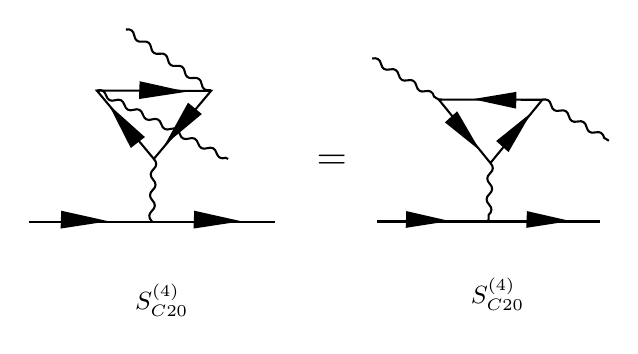
\begin{tikzpicture}[x=0.75pt,y=0.75pt,yscale=-1,xscale=1]
%uncomment if require: \path (0,267); %set diagram left start at 0, and has height of 267

%Shape: Triangle [id:dp4403355990984392] 
\draw   (161.28,103.91) -- (133.84,71.01) -- (188.86,71.13) -- cycle ;
%Straight Lines [id:da5357747567650413] 
\draw    (101,134.24) -- (219.5,134.24) ;
%Straight Lines [id:da3607994343394286] 
\draw    (161.28,103.91) .. controls (162.89,105.63) and (162.83,107.29) .. (161.11,108.9) .. controls (159.39,110.51) and (159.33,112.18) .. (160.94,113.9) .. controls (162.55,115.62) and (162.49,117.29) .. (160.77,118.9) .. controls (159.05,120.51) and (158.99,122.17) .. (160.6,123.89) .. controls (162.21,125.61) and (162.15,127.28) .. (160.43,128.89) .. controls (158.71,130.5) and (158.65,132.17) .. (160.26,133.89) -- (160.25,134.24) -- (160.25,134.24) ;
%Straight Lines [id:da2551423225028494] 
\draw    (133.84,71.01) .. controls (136.09,70.3) and (137.57,71.07) .. (138.28,73.32) .. controls (138.99,75.57) and (140.46,76.34) .. (142.71,75.63) .. controls (144.96,74.92) and (146.43,75.69) .. (147.14,77.94) .. controls (147.85,80.19) and (149.33,80.97) .. (151.58,80.26) .. controls (153.83,79.55) and (155.3,80.32) .. (156.01,82.57) .. controls (156.72,84.82) and (158.2,85.59) .. (160.45,84.88) .. controls (162.7,84.17) and (164.17,84.94) .. (164.88,87.19) .. controls (165.59,89.44) and (167.06,90.21) .. (169.31,89.5) .. controls (171.56,88.79) and (173.04,89.56) .. (173.75,91.81) .. controls (174.46,94.06) and (175.93,94.83) .. (178.18,94.12) .. controls (180.43,93.41) and (181.9,94.18) .. (182.61,96.43) .. controls (183.32,98.68) and (184.8,99.46) .. (187.05,98.75) .. controls (189.3,98.04) and (190.77,98.81) .. (191.48,101.06) .. controls (192.19,103.31) and (193.67,104.08) .. (195.92,103.37) -- (197.07,103.97) -- (197.07,103.97) ;
%Straight Lines [id:da36371740519141016] 
\draw    (147.8,41.57) .. controls (150.13,41.19) and (151.48,42.16) .. (151.86,44.49) .. controls (152.24,46.82) and (153.59,47.79) .. (155.92,47.41) .. controls (158.25,47.03) and (159.6,48) .. (159.97,50.33) .. controls (160.35,52.66) and (161.7,53.63) .. (164.03,53.25) .. controls (166.36,52.87) and (167.71,53.84) .. (168.09,56.17) .. controls (168.47,58.5) and (169.82,59.47) .. (172.15,59.1) .. controls (174.48,58.72) and (175.83,59.69) .. (176.21,62.02) .. controls (176.58,64.35) and (177.93,65.32) .. (180.26,64.94) .. controls (182.59,64.56) and (183.94,65.53) .. (184.32,67.86) .. controls (184.7,70.19) and (186.05,71.16) .. (188.38,70.78) -- (188.86,71.13) -- (188.86,71.13) ;
%Shape: Triangle [id:dp17894578128011973] 
\draw  [fill={rgb, 255:red, 0; green, 0; blue, 0 }  ,fill opacity=1 ] (136.71,133.86) -- (116.89,136.89) -- (117.14,129.5) -- cycle ;
%Shape: Triangle [id:dp06076395640370147] 
\draw  [fill={rgb, 255:red, 0; green, 0; blue, 0 }  ,fill opacity=1 ] (200.76,133.86) -- (180.94,136.89) -- (181.19,129.5) -- cycle ;
%Shape: Triangle [id:dp8878620023930338] 
\draw  [fill={rgb, 255:red, 0; green, 0; blue, 0 }  ,fill opacity=1 ] (174.48,71.46) -- (154.66,74.48) -- (154.91,67.1) -- cycle ;
%Shape: Triangle [id:dp8358689677471037] 
\draw  [fill={rgb, 255:red, 0; green, 0; blue, 0 }  ,fill opacity=1 ] (168.21,95.14) -- (177.91,77.6) -- (183.61,82.3) -- cycle ;
%Shape: Triangle [id:dp7541281922212124] 
\draw  [fill={rgb, 255:red, 0; green, 0; blue, 0 }  ,fill opacity=1 ] (141.26,79.99) -- (156.2,93.36) -- (150.34,97.87) -- cycle ;
%Shape: Triangle [id:dp2775236183570764] 
\draw   (323.44,105.89) -- (298.54,75.31) -- (348.46,75.42) -- cycle ;
%Straight Lines [id:da9722316781434073] 
\draw    (268.74,134.09) -- (376.27,134.09) ;
%Straight Lines [id:da8593434245871657] 
\draw    (323.44,105.89) .. controls (325.05,107.61) and (324.99,109.28) .. (323.27,110.89) .. controls (321.55,112.5) and (321.5,114.16) .. (323.11,115.88) .. controls (324.72,117.6) and (324.66,119.27) .. (322.94,120.88) .. controls (321.22,122.49) and (321.16,124.16) .. (322.77,125.88) .. controls (324.38,127.6) and (324.33,129.27) .. (322.61,130.88) -- (322.5,134.09) -- (322.5,134.09) ;
%Straight Lines [id:da6801121149920226] 
\draw    (266.5,55.57) .. controls (268.79,55.02) and (270.21,55.9) .. (270.76,58.19) .. controls (271.3,60.48) and (272.72,61.36) .. (275.01,60.81) .. controls (277.3,60.26) and (278.72,61.14) .. (279.27,63.43) .. controls (279.82,65.72) and (281.24,66.6) .. (283.53,66.06) .. controls (285.82,65.51) and (287.24,66.39) .. (287.78,68.68) .. controls (288.33,70.97) and (289.75,71.85) .. (292.04,71.3) .. controls (294.33,70.76) and (295.75,71.64) .. (296.3,73.93) -- (298.54,75.31) -- (298.54,75.31) ;
%Straight Lines [id:da6825232417758785] 
\draw    (348.46,75.41) .. controls (350.75,74.87) and (352.17,75.75) .. (352.72,78.04) .. controls (353.26,80.33) and (354.68,81.21) .. (356.97,80.66) .. controls (359.26,80.11) and (360.68,80.99) .. (361.23,83.28) .. controls (361.78,85.57) and (363.2,86.45) .. (365.49,85.9) .. controls (367.78,85.36) and (369.2,86.24) .. (369.75,88.53) .. controls (370.29,90.82) and (371.71,91.7) .. (374,91.15) .. controls (376.29,90.6) and (377.71,91.48) .. (378.26,93.77) -- (380.5,95.15) -- (380.5,95.15) ;
%Shape: Triangle [id:dp9388080791708642] 
\draw  [fill={rgb, 255:red, 0; green, 0; blue, 0 }  ,fill opacity=1 ] (301.14,133.74) -- (283.16,136.55) -- (283.38,129.68) -- cycle ;
%Shape: Triangle [id:dp1748578963133881] 
\draw  [fill={rgb, 255:red, 0; green, 0; blue, 0 }  ,fill opacity=1 ] (359.26,133.74) -- (341.27,136.55) -- (341.5,129.68) -- cycle ;
%Shape: Triangle [id:dp15147480418604864] 
\draw  [fill={rgb, 255:red, 0; green, 0; blue, 0 }  ,fill opacity=1 ] (317.54,75.19) -- (335.5,72.2) -- (335.34,79.07) -- cycle ;
%Shape: Triangle [id:dp570772188769084] 
\draw  [fill={rgb, 255:red, 0; green, 0; blue, 0 }  ,fill opacity=1 ] (341.32,83.79) -- (332.04,99.83) -- (327,95.31) -- cycle ;
%Shape: Triangle [id:dp661357960588842] 
\draw  [fill={rgb, 255:red, 0; green, 0; blue, 0 }  ,fill opacity=1 ] (316.64,97.81) -- (302.29,86.3) -- (307.32,81.77) -- cycle ;

% Text Node
\draw (165.04,172.01) node  [font=\small]  {$S^{( 4)}_{C20}$};
% Text Node
\draw (326.85,169.2) node  [font=\small]  {$S^{( 4)}_{C20}$};
% Text Node
\draw (247,105.57) node  [font=\Large] [align=left] {=};


\end{tikzpicture}
    \caption{Equivalent Triangle Diagrams}
    \label{fig:equivalent-triangle}
\end{figure}
\bluep{\textbf{Recall from the derivation of the Dirac particle propagator that the propagator for an anti-fermion has the opposite sign of the fermion. So switching fermion and anti-fermion propagators introduces a minus sign into the total amplitude for each such switch.}} There are three switches from the RHS of Fig.\ref{fig:equivalent-triangle} to the next to last diagram in Fig.\ref{fig:compton-tree-2nd}. Since $(-1)^3=-1$, the amplitude for the two diagrams are the same except for sign. So when added, \textbf{\redp{they cancel exactly, and we don't have to consider them anymore.}}
\begin{qt}
    \underline{Furry's Theorem:} Diagrams containing an all fermion sided polygon having an odd number of sides always occur in pairs, and the contributions of such pairs to the total amplitude cancel out.
\end{qt}

\begin{qt}
    \textbf{Only reducible diagrams yield divergent integrals and thus, divergent amplitudes}.
\end{qt}

\section{Renormalizing 2nd Order Divergent Amplitudes}
\subsection{Steps of Renormalization}
